% !Mode:: "TeX:UTF-8"
% \textbf{类比探究专练之中点结构(一)}
% T22(题号)-A(难度ABC)03(序号)

\begin{defproblem}{T22-A03-01}%
\begin{onlyproblem}%
\href{run:./ItemBankFigures/T22-A03-01.ggb}{(查看动态演示)}
如图1,点$E$是正方形$ABCD$边$CD$上任意一点,以$DE$为边作正方形$DEFG$,连接$BF$,点$M$是线段$BF$中点,射线$EM$与$BC$交于点$H$,连接$CM$.

(1)请直接写出$CM$和$EM$的数量关系和位置关系.

(2)把图1中的正方形$DEFG$绕点$D$顺时针旋转45$^{\circ }$,此时点$F$恰好落在线段$CD$上,如图2,其他条件不变,(1)中的结论是否成立?请说明理由.

(3)把图1中的正方形$DEFG$绕点$D$顺时针旋转90$^{\circ }$,此时点$E$,$G$恰好分别落在线段$AD$,$CD$上,如图3,其他条件不变,(1)中的结论是否成立?请说明理由.
\begin{center}
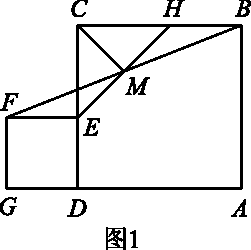
\includegraphics[scale=0.8]{T22-A03-01.pdf}\qquad
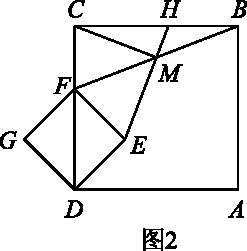
\includegraphics[scale=0.8]{T22-A03-02.pdf}\qquad
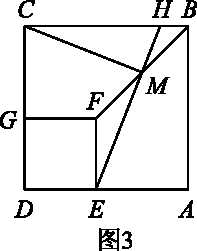
\includegraphics[scale=0.8]{T22-A03-03.pdf}
\end{center}
% \begin{flushright}
% 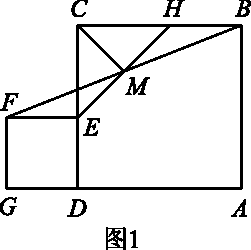
\includegraphics[scale=0.8]{T22-A03-01.pdf}\\
% 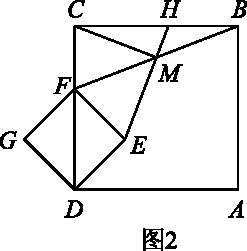
\includegraphics[scale=0.8]{T22-A03-02.pdf}\\
% 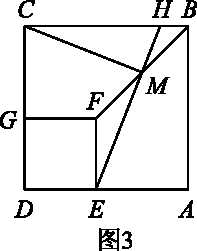
\includegraphics[scale=0.8]{T22-A03-03.pdf}
% \end{flushright}

\end{onlyproblem}%
\begin{onlysolution}%
解决类比探究问题的一般方法:

1.	若属于类比探究常见的结构类型,调用结构类比解决.

类比探究结构举例:旋转结构、中点结构.

2.	若不属于常见结构类型

①根据题干条件,结合\underline{\hspace*{3cm}}先解决第一问.

②类比解决下一问.

如果不能,分析条件变化,寻找\underline{\hspace*{3cm}}.
结合所求目标,依据\underline{\hspace*{3cm}},大胆猜测、尝试、验证.


\begin{center}
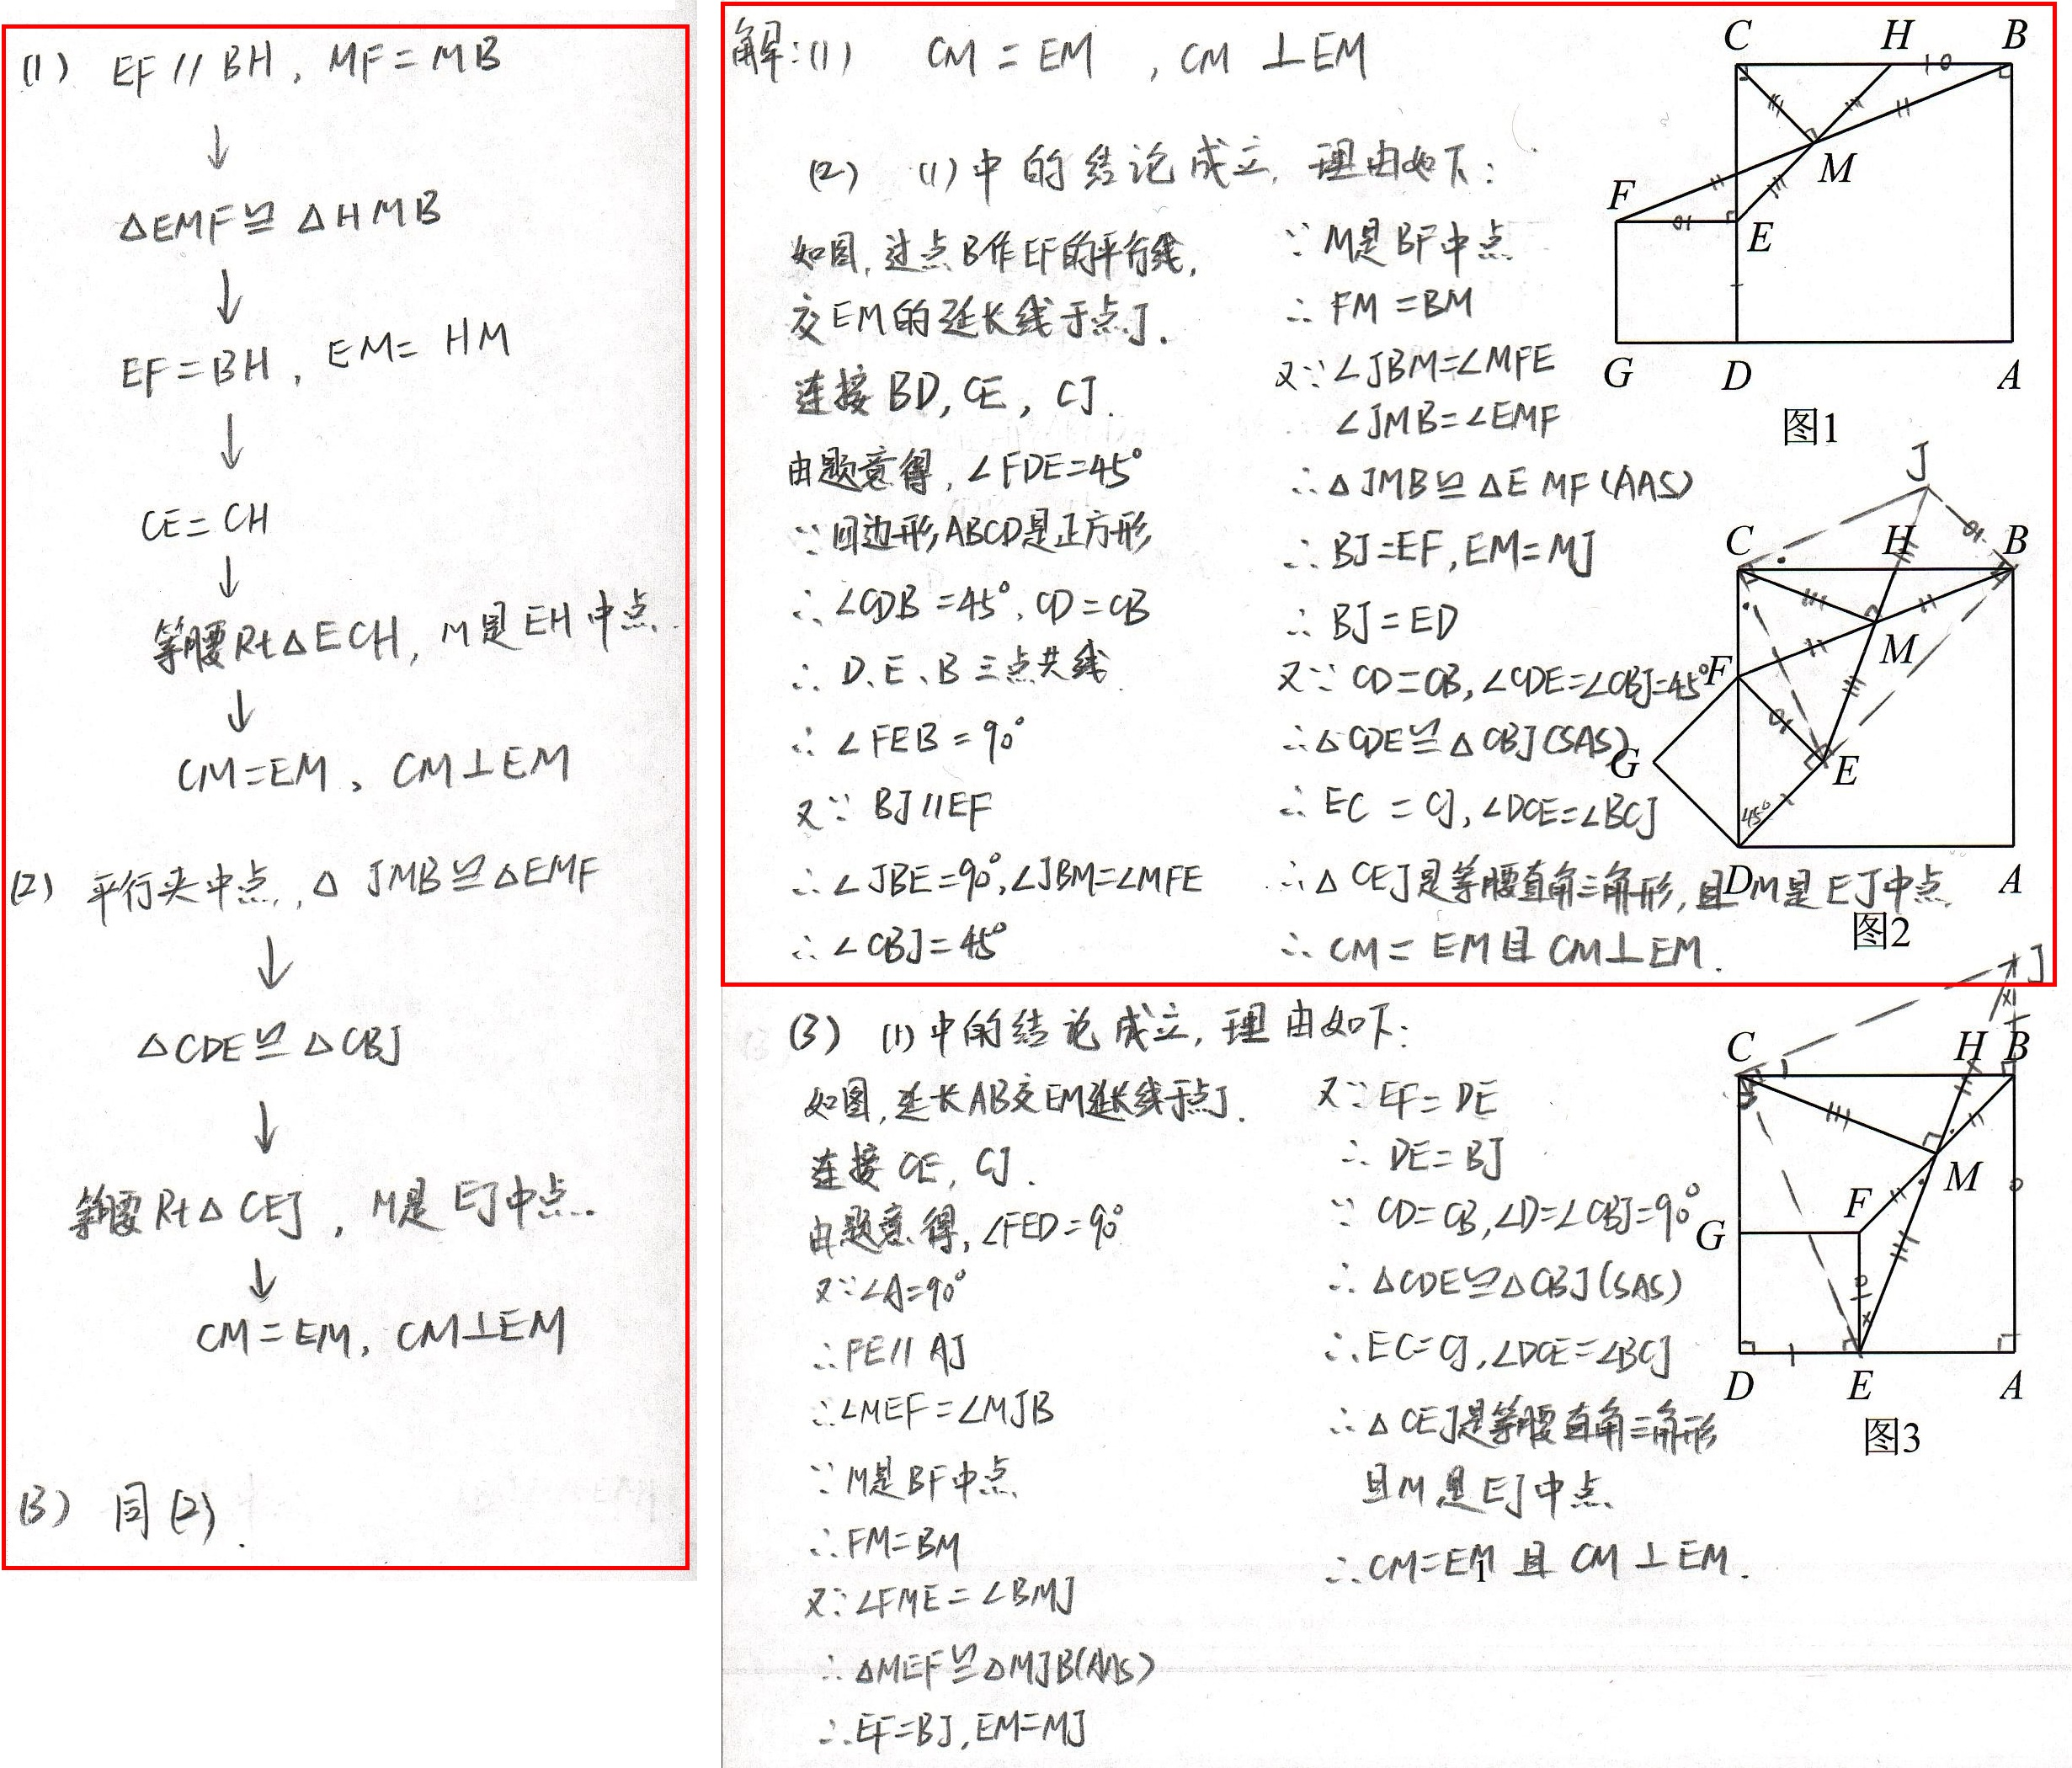
\includegraphics[width=.95\textwidth]{T22-A03-04-Ans.jpg}
\end{center}
\end{onlysolution}%
\end{defproblem}





\begin{defproblem}{T22-A03-02}%
\begin{onlyproblem}%
% \href{run:./ItemBankFigures/T22-A01-06.ggb}{(查看动态演示)}
在菱形$ABCD$和正三角形$BGF$中,$\angle $$ABC$=60$^{\circ }$,$P$是$DF$的中点,连接$PG$,$PC$.如图1,当点$G$在$BC$边上时,易证:$PG=\sqrt 3 PC$(不必证明).

(1)如图2,当点$F$在$AB$的延长线上时,线段$PC$,$PG$有怎样的数量关系?写出你的猜想,并给予证明;

(2)如图3,当点$F$在$CB$的延长线上时,线段$PC$,$PG$又有怎样的数量关系?请写出你的猜想(不必证明).


\begin{center}
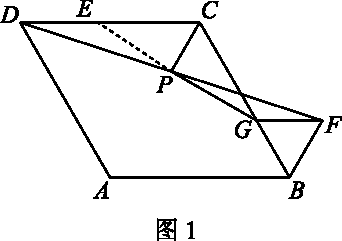
\includegraphics[scale=0.78]{T22-A03-02-01.pdf}\qquad
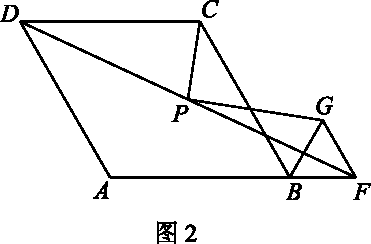
\includegraphics[scale=0.78]{T22-A03-02-02.pdf}\qquad
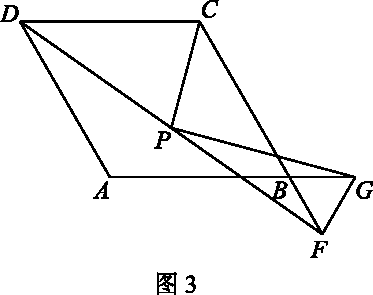
\includegraphics[scale=0.78]{T22-A03-02-03.pdf}
\end{center}


% \begin{flushright}
% 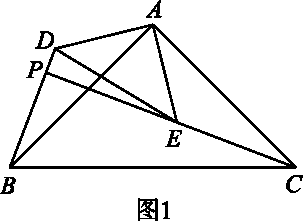
\includegraphics[scale=0.8]{T22-A01-02-01.pdf}\\
% 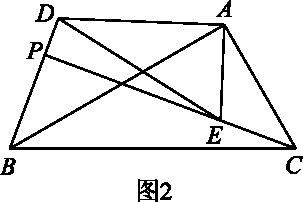
\includegraphics[scale=0.8]{T22-A01-02-02.pdf}\\
% 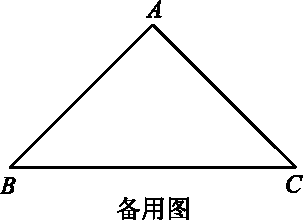
\includegraphics[scale=0.8]{T22-A01-02-03.pdf}
% \end{flushright}

\end{onlyproblem}%
\begin{onlysolution}%
(1)$P G=\sqrt{3} P C$,证明略.

提示:延长$GP$,交$AD$于点$E$.

证明$\triangle DEP\cong \triangle FGP$(ASA),得到$PG=PE$,$DE=FG$,

证明$\triangle CED\cong\triangle CGB$(SAS),得到$CE=CG$,

由三线合一得,$PG \bot PC$,进而可得$P G=\sqrt{3} P C$.

(2)$P G=\sqrt{3} P C$

\begin{center}
% 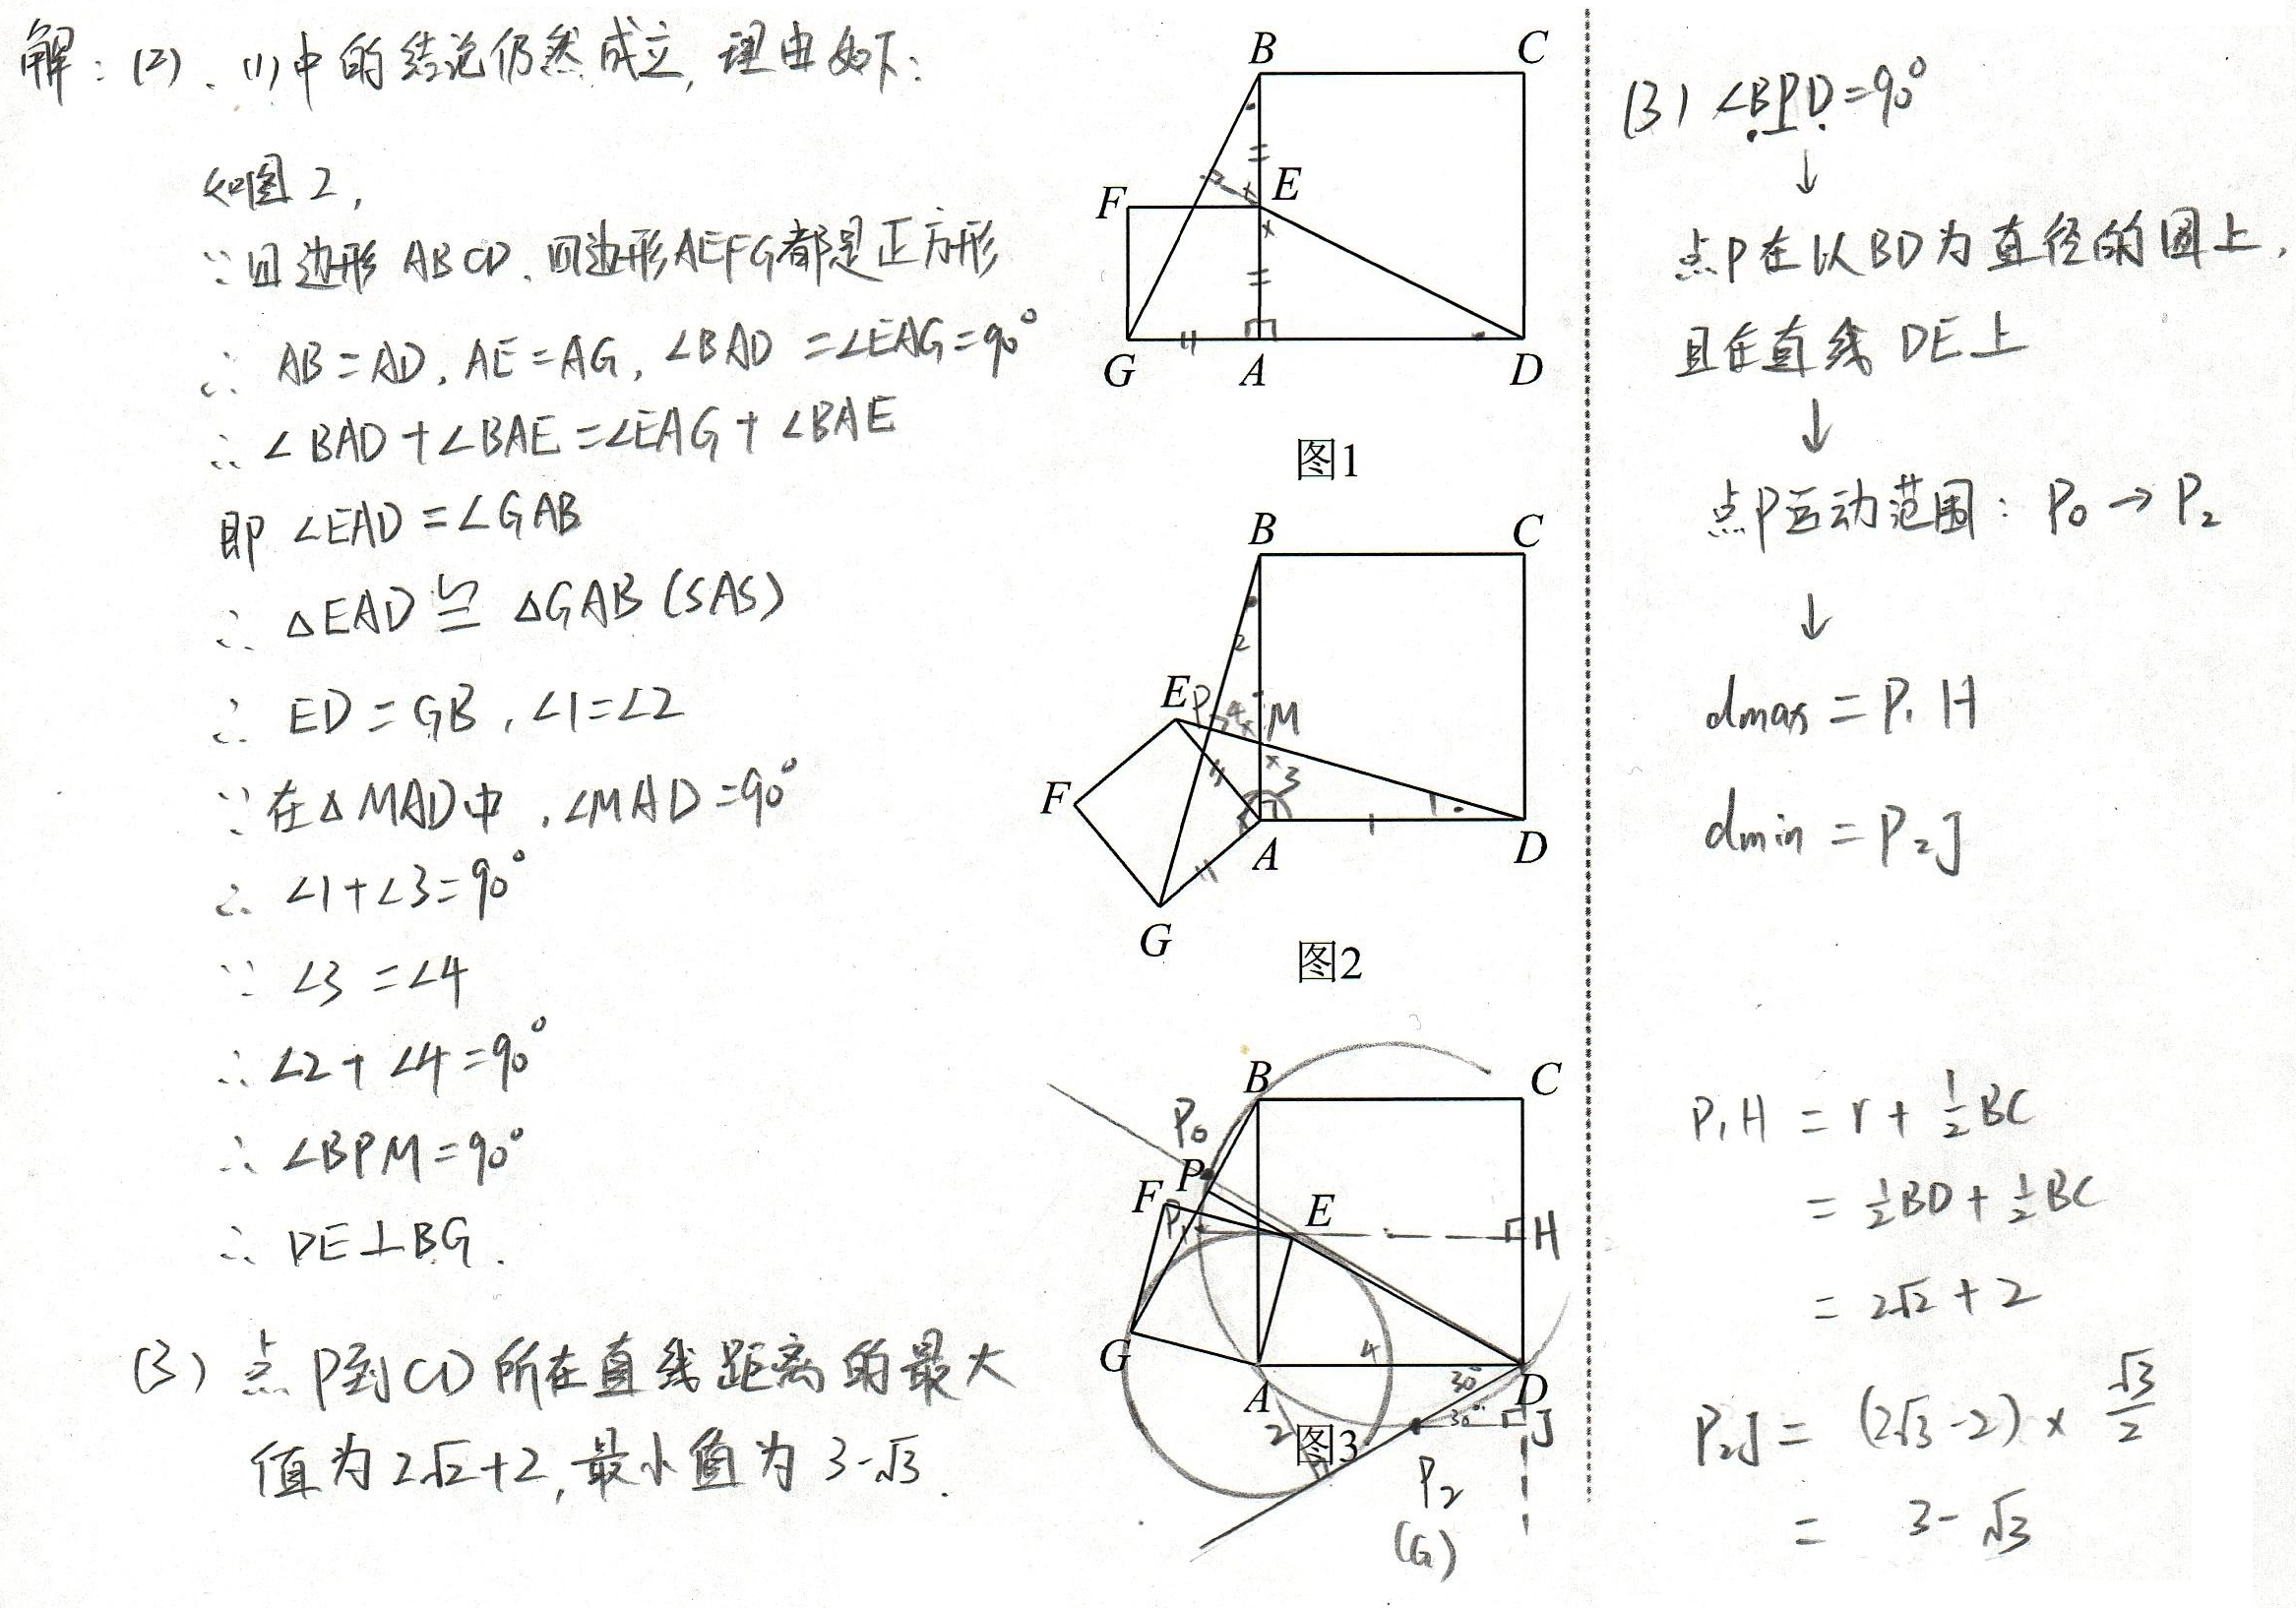
\includegraphics[width=.95\textwidth]{T22-A01-06-04-Ans.jpg}
\end{center}
\end{onlysolution}%
\end{defproblem}



\begin{defproblem}{T22-A03-03}%
\begin{onlyproblem}%
\href{run:./ItemBankFigures/T22-A03-03.ggb}{(查看动态演示)}
已知,在正方形$ABCD$中,$\triangle BEF$是以$BF$为斜边的等腰直角三角形,取$DF$的中点$G$,连接$EG$,$CG$.

(1)如图1,若$\triangle BEF$的斜边$BF$在$BC$上,猜想$EG$和$CG$之间的数量关系,并证明.

(2)将图1中的$\triangle BEF$绕点$B$顺时针旋转45$^{\circ }$,如图2所示,则(1)中的结论是否仍成立?若成立,请给出证明;若不成立,请说明理由.

(3)将图1中的$\triangle BEF$绕点$B$顺时针旋转任意角度,如图3所示,则(1)中的结论是否仍成立?若成立,请给出证明;若不成立,请说明理由.


\begin{center}
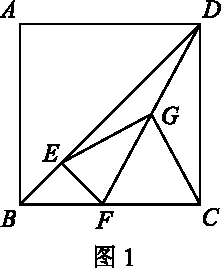
\includegraphics[scale=0.8]{T22-A03-03-01.pdf}\qquad
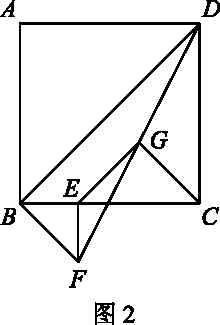
\includegraphics[scale=0.8]{T22-A03-03-02.pdf}\qquad
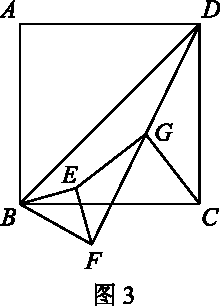
\includegraphics[scale=0.8]{T22-A03-03-03.pdf}
\end{center}


% \begin{flushright}
% 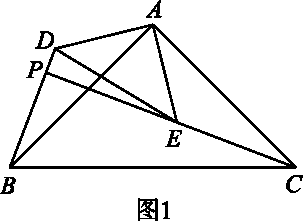
\includegraphics[scale=0.8]{T22-A01-02-01.pdf}\\
% 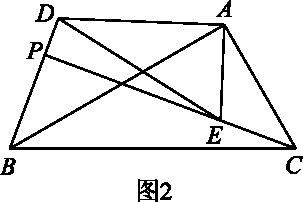
\includegraphics[scale=0.8]{T22-A01-02-02.pdf}\\
% 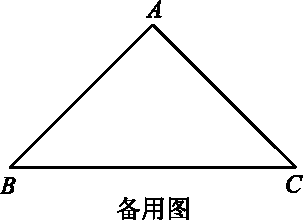
\includegraphics[scale=0.8]{T22-A01-02-03.pdf}
% \end{flushright}

\end{onlyproblem}%
\begin{onlysolution}%
(1)$EG=CG$,证明略.

提示:直角三角形斜边中线等于斜边的一半.

(2)(1)中的结论仍成立,证明略.

提示:延长$EG$,交$CD$于点$H$.

证明$\triangle EFG\cong \triangle HDG$(ASA),得到$EF=HD$,$EG=HG$,再由直角三角形斜边中线等于斜边的一半即可得证.

(3)(1)中的结论仍成立,证明略.

提示:过点$D$作$DH//EF$,交$EG$的延长线于点$H$,连接$CE$,$CH$.

\begin{center}
% 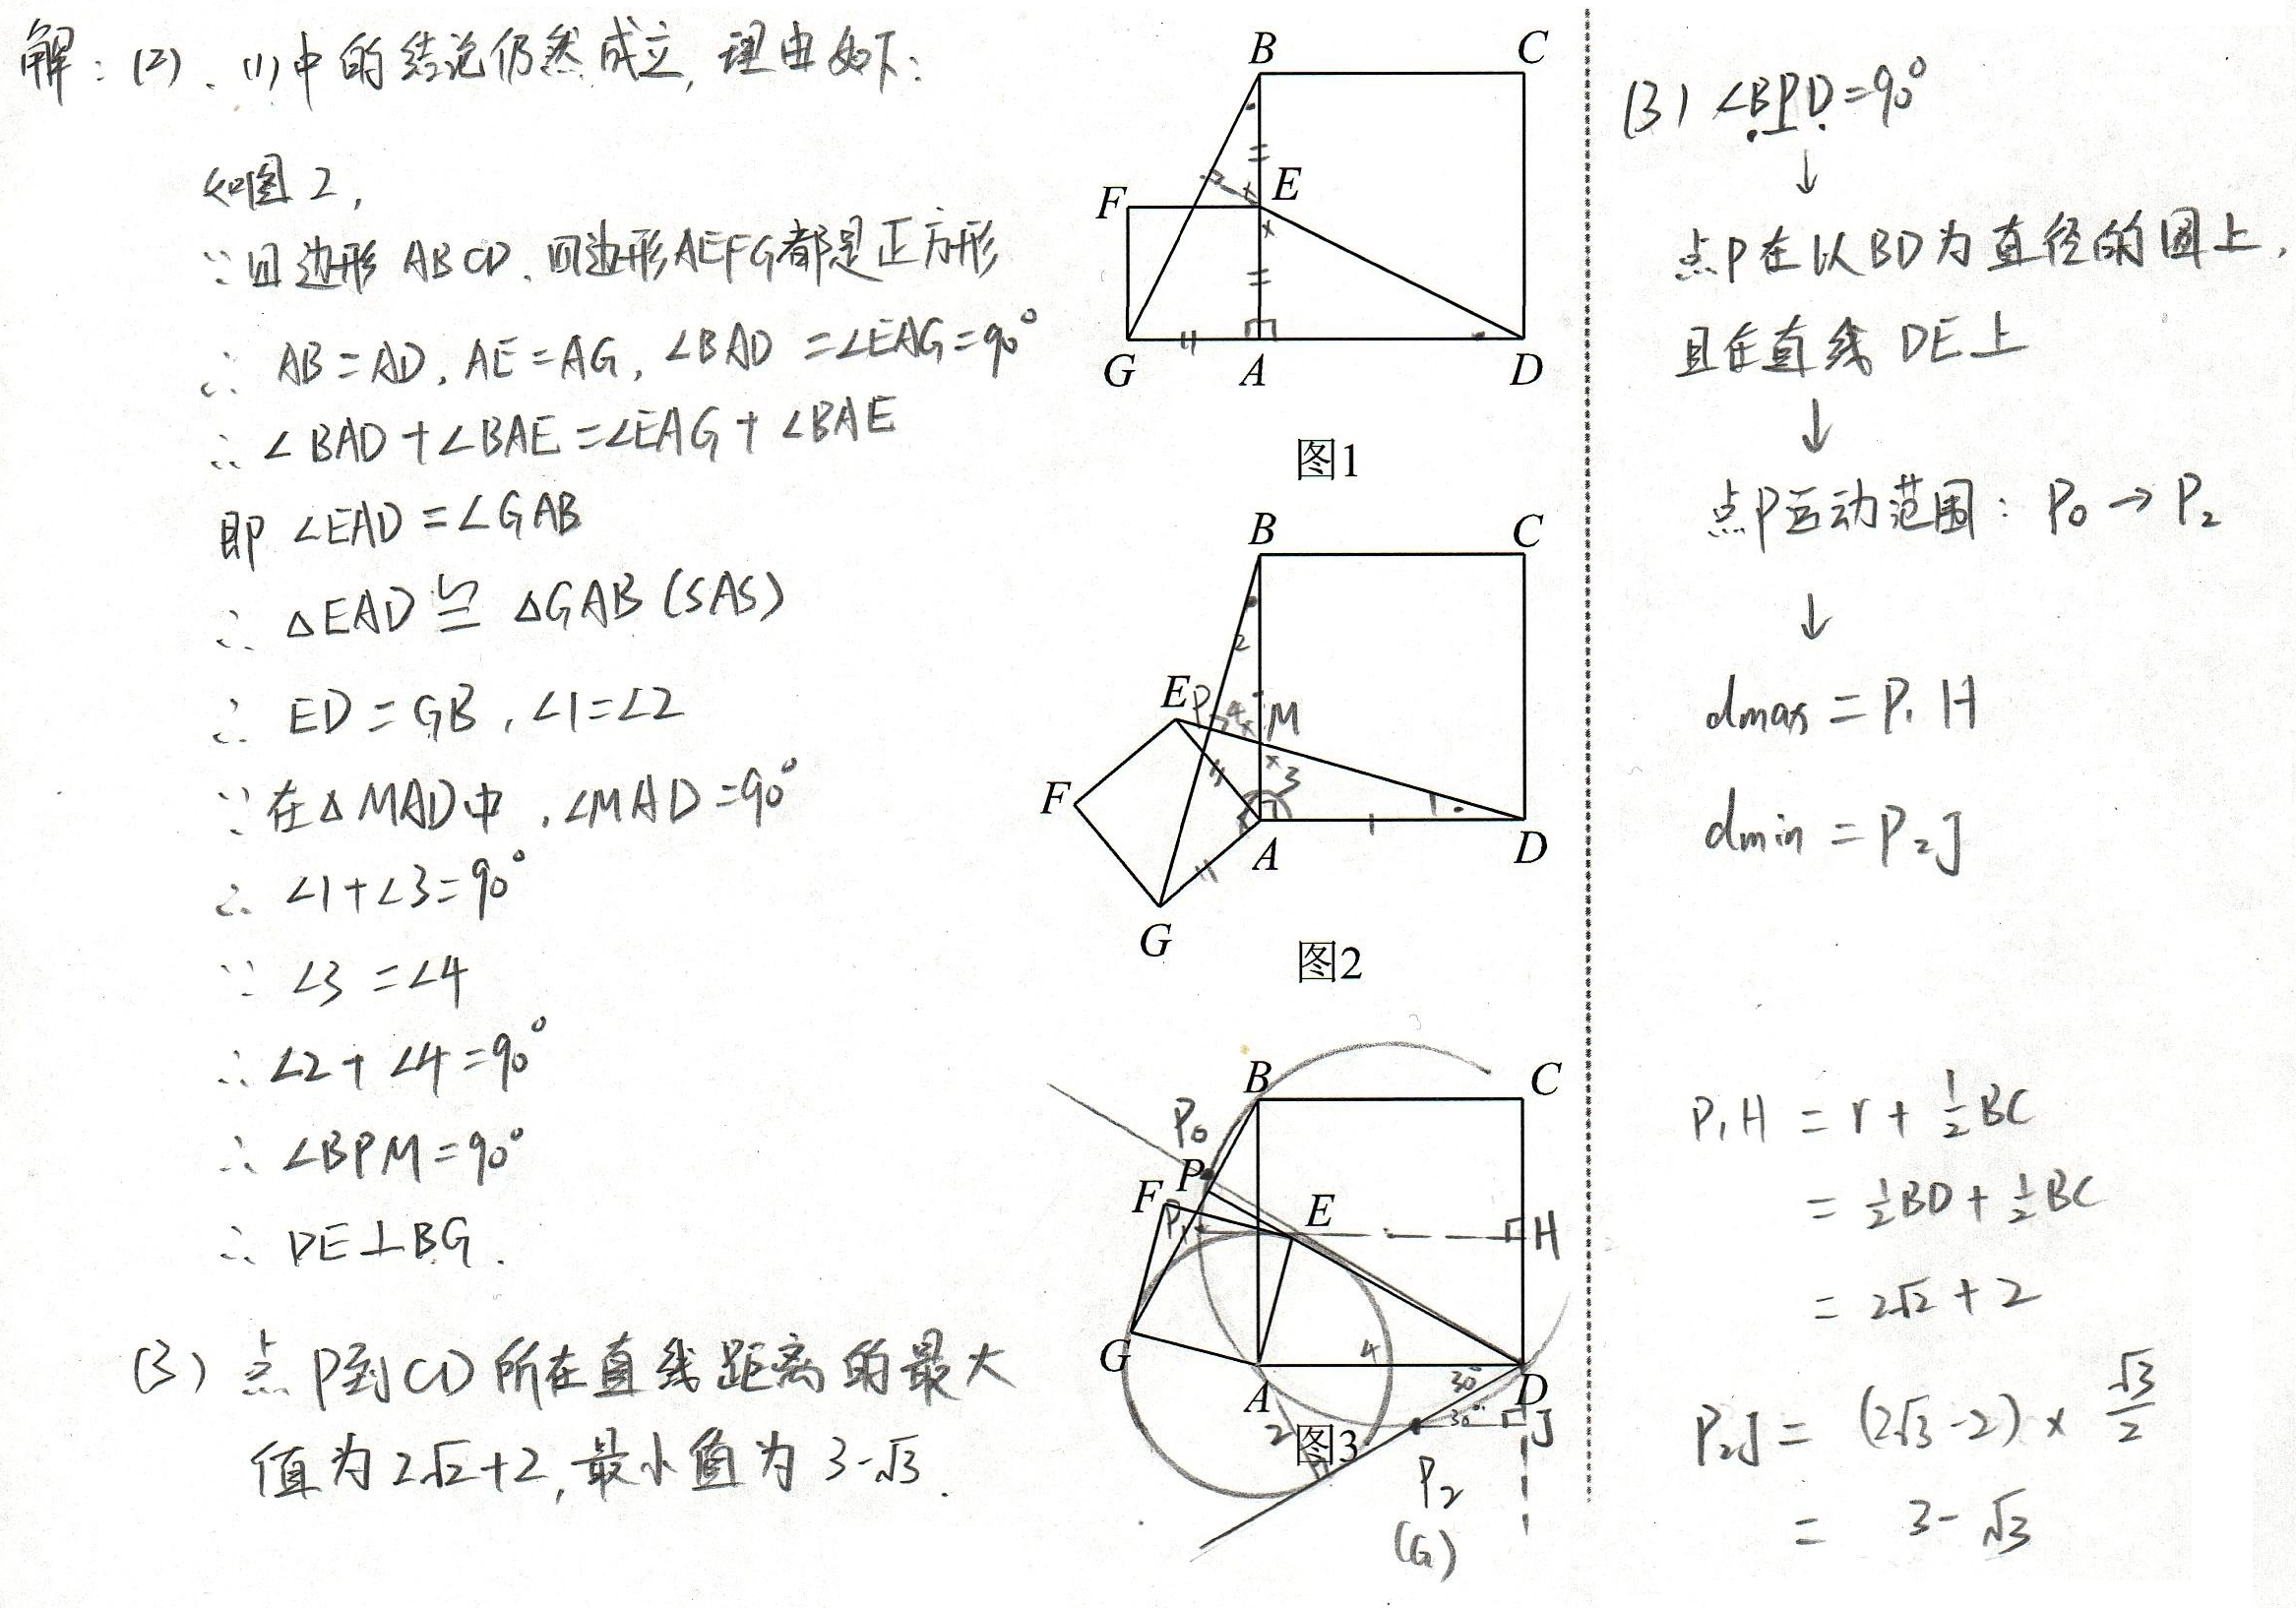
\includegraphics[width=.95\textwidth]{T22-A01-06-04-Ans.jpg}
\end{center}
\end{onlysolution}%
\end{defproblem}
